% !TeX root = main.tex
% Converted from chapter-three-revision-2026-10-17.md; source notes retained separately.
\chapter{Methodology and System Design}\label{chap:3}

\section{Introduction}\label{sec:3-1}

The project adopts an engineering design and development approach with iterative prototyping and experimental evaluation. Development is organised around requirements, records and document design, web application development, terminal implementation, integration and testing. The filing system is treated as the foundation of the application, while fingerprint recognition supplies identity evidence for selected departmental activities.

The methodology addresses the two research questions established in Chapter One. The first concerns the organisation, controlled updating and retrieval of structured records and uploaded documents. The second concerns the association of fingerprint evidence with the appropriate student record and its use within a reliable workflow. Separate subsystem tests and integration tests are used because a functioning scanner or backend alone does not establish the behaviour of the complete application.

\section{Study Context and Requirements}\label{sec:3-2}

\subsection{Departmental context and information sources}\label{sec:3-2-1}

The project concerns student filing and management in the Department of Electrical and Electronic Engineering, Obafemi Awolowo University. The H.O.D. (Head of Department) reported on 23 September 2026 that records are predominantly hard copies, are difficult to retrieve, and require considerable effort to review, update and correct. The H.O.D. also confirmed that the filing system includes both structured records and uploaded documents.

This clarification provides a requirements input and a local description of the problem. It is not treated as a quantified retrieval-time study or a completed programme of stakeholder interviews. Requirements were further informed by the supplied literature, the team's recorded software and attendance decisions, the existing data models and API contracts, and the documented hardware feasibility work. A fuller process description remains necessary to establish record categories, custody, indexing and departmental correction authority.

The literature was reviewed by separating project drafts from reference publications and checking whether the latter supported the claims attributed to them. Hardware descriptions were reconciled with the actual terminal records. This process informed the filing-first structure of the system and removed unsupported assumptions about recognition accuracy, component specifications and completed network integration.

\subsection{Functional requirements}\label{sec:3-2-2}

Table 3.1 defines the principal requirements. Implementation status refers to the development evidence available for this draft, rather than to production deployment.


% !TeX root = ../main.tex
\begingroup
\singlespacing%
\setlength{\tabcolsep}{4pt}
\begin{longtable}{@{}>{\RaggedRight\arraybackslash}p{\dimexpr0.220\linewidth-2\tabcolsep\relax}>{\RaggedRight\arraybackslash}p{\dimexpr0.390\linewidth-2\tabcolsep\relax}>{\RaggedRight\arraybackslash}p{\dimexpr0.390\linewidth-2\tabcolsep\relax}@{}}
\caption{Principal system requirements and implementation position}\label{tab:3-1}\\
\toprule
\textbf{ID} & \textbf{Requirement} & \textbf{Implementation position} \\
\midrule
\endfirsthead%
\toprule
\textbf{ID} & \textbf{Requirement} & \textbf{Implementation position} \\
\midrule
\endhead%
\midrule
\multicolumn{3}{r}{Continued on next page}\\
\endfoot%
\bottomrule
\endlastfoot%
R1 & Maintain a stable student identity with validated profile and academic information & Backend models and controlled operations implemented. \\ \addlinespace
R2 & Search and retrieve the permitted student and academic records & Backend APIs implemented; connected browser workflow still requires validation. \\ \addlinespace
R3 & Upload, classify, associate and retrieve supporting documents privately & Confirmed scope; document-storage implementation remains proposed. \\ \addlinespace
R4 & Control corrections and preserve the relevant academic or document history & Academic rules and selected history mechanisms exist; document revision history and comprehensive audit remain incomplete. \\ \addlinespace
R5 & Enforce user permissions and adviser, course or ownership scope & Backend access mechanisms implemented for the corresponding operations. \\ \addlinespace
R6 & Acquire fingerprints and carry out the supported recognition experiments & Diagnostic, recognition-pilot and deferred-capture firmware paths implemented; their test contexts are distinct. \\ \addlinespace
R7 & Associate an enrolled biometric identity with the permanent student record & Restricted enrolment/binding and integrated resolution remain to be completed. \\ \addlinespace
R8 & Preserve offline captures and transfer them without losing event identity & Device storage, USB export and pending backend ingestion implemented. \\ \addlinespace
R9 & Apply identity, roster, timing and permission checks before biometric attendance is recorded & Attendance and roster foundations exist; complete biometric reconciliation remains proposed. \\ \addlinespace
R10 & Produce evidence of correctness, timing and selected failure behaviour & Subsystem and backend evidence exists; records-task, document and full integration evaluations remain to be completed. \\ \addlinespace
\end{longtable}
\endgroup


\subsection{Non-functional requirements}\label{sec:3-2-3}

The system requires consistent records, bounded processing, controlled disclosure and recoverable operation. Invalid or conflicting input should be rejected without leaving a partial update. A repeated submission should preserve the identity of the original operation. Missing identity or timing information should remain unresolved rather than being converted into an assumed attendance decision.

Performance is evaluated through defined timing intervals and datasets. No institutional retrieval-time target or population biometric-accuracy target has been established by the present requirements material. These targets must be agreed before any final acceptance study that depends on them. Functional acceptance can nevertheless be specified precisely: a permitted request must return the correct record, a denied request must not disclose it, and a rejected transaction must leave the protected state unchanged.

\section{Development Procedure and System Architecture}\label{sec:3-3}

\subsection{Iterative development procedure}\label{sec:3-3-1}

Development proceeded through successive records/backend, terminal and integration increments. The software work established student and academic entities, access policies and controlled services. Hardware work established scanner communication, reference transfer, recognition experiments and persistent unidentified capture. The later backend increment introduced authorised preview and ingestion of capture batches while keeping them pending identity and timing review.

The remaining increments concern private document management, restricted biometric identity binding, reviewed reconciliation and connected browser operation. Each increment is evaluated against its requirements before its behaviour is described as a completed system function. This approach permits faults discovered through subsystem, HTTP or database tests to inform the next revision without implying that all development followed a single uninterrupted sequence.

\subsection{Logical architecture}\label{sec:3-3-2}

The records application separates browser presentation, backend services and persistent data. Django and Django REST Framework implement the current backend. Structured records are represented through Django models and migrations. PostgreSQL is the intended application database and has been used in isolated integration validation; SQLite has also been used for isolated development tests. Shared-source reconciliation and production database cutover are separate activities.

The browser interface is a client of the backend rather than a direct database client. 
%The reviewed frontend folder contains prototypes; their demonstration state is not evidence of complete API integration. 
The proposed document subsystem adds metadata management and private file storage to the existing structured-record services.

Figure 3.1 distinguishes the implemented deferred-capture route from the remaining integration. Solid arrows show established logical interfaces; dashed arrows identify proposed components or connections. The diagram does not assert completed browser integration or direct device-to-server Wi-Fi transfer.

\begin{figure}[htbp]
\centering
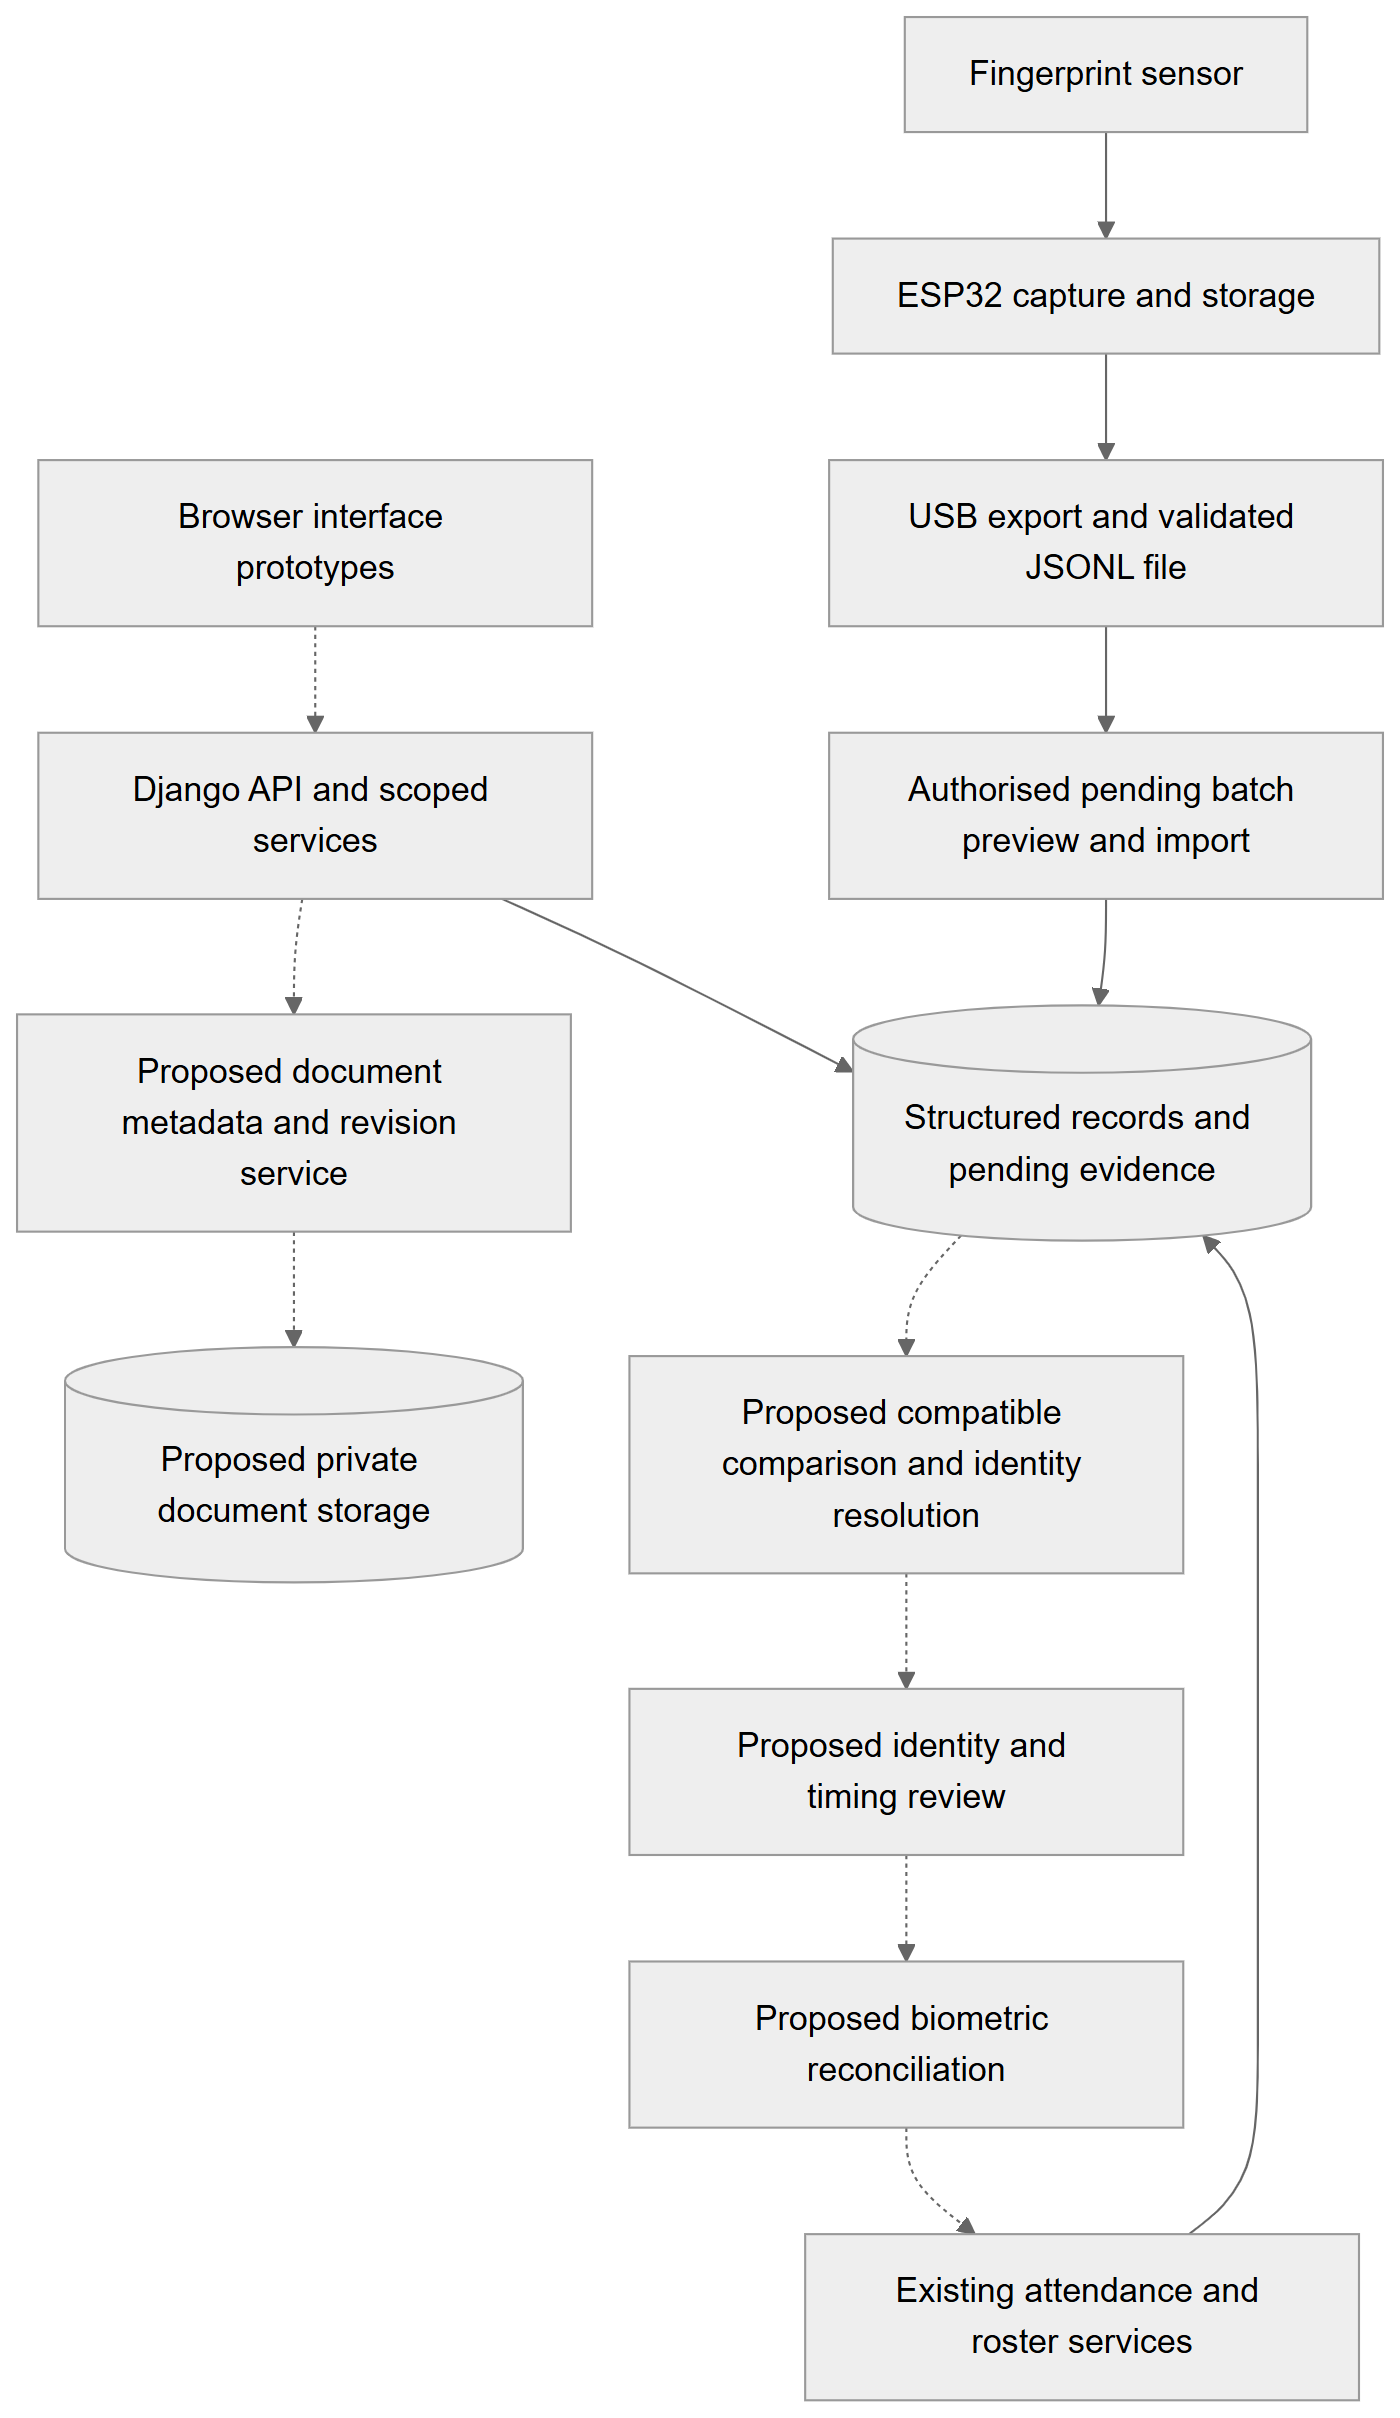
\includegraphics[width=\linewidth,height=0.78\textheight,keepaspectratio]{folder/figure-3_1-system-architecture.png}
\caption{System architecture with implemented and proposed connections}\label{fig:3-1}
\end{figure}
\clearpage

The design keeps the identity and records responsibilities explicit. The database can store pending biometric evidence before it can interpret that evidence as a student identity. Private document storage similarly requires its own access and consistency rules rather than being implied by the presence of student tables.

\section{Records and Database Design}\label{sec:3-4}

\subsection{Student identity and core entities}\label{sec:3-4-1}

The implemented Student model uses a permanent UUID as its primary identifier. Matriculation or UTME information is stored as a separate textual identifier, preserving leading zeros and allowing the student's internal identity to remain stable. An optional account link associates a login user with a student profile. Guardians are separate records linked to the student.

Academic information is organised through sessions, courses, course offerings and result attempts. A course offering associates a course with a session, semester, level, credit units and grading scale. A result links a student to an offering and an attempt number. It also retains the credit units and grading reference needed for the historical calculation.


% !TeX root = ../main.tex
\begingroup
\singlespacing%
\setlength{\tabcolsep}{4pt}
\begin{longtable}{@{}>{\RaggedRight\arraybackslash}p{\dimexpr0.220\linewidth-2\tabcolsep\relax}>{\RaggedRight\arraybackslash}p{\dimexpr0.390\linewidth-2\tabcolsep\relax}>{\RaggedRight\arraybackslash}p{\dimexpr0.390\linewidth-2\tabcolsep\relax}@{}}
\caption{Selected implemented records and integrity rules}\label{tab:3-2}\\
\toprule
\textbf{Entity} & \textbf{Principal information} & \textbf{Important relationship or rule} \\
\midrule
\endfirsthead%
\toprule
\textbf{Entity} & \textbf{Principal information} & \textbf{Important relationship or rule} \\
\midrule
\endhead%
\midrule
\multicolumn{3}{r}{Continued on next page}\\
\endfoot%
\bottomrule
\endlastfoot%
Student & Permanent UUID, external identifier, name, admission and current academic information & External identifier is unique; account linkage is optional and one-to-one. \\ \addlinespace
Guardian & Name, relationship and contact information & Linked to a student; several guardian records may belong to the same student. \\ \addlinespace
Academic\allowbreak~Session & Academic-year label & Unique session with a validated consecutive-year format. \\ \addlinespace
Course & Course code and title & Course code is unique. \\ \addlinespace
Course\allowbreak~Offering & Course, session, semester, level, units and grading scale & Course/session/semester combination is unique. \\ \addlinespace
Result & Student, offering, attempt, score, saved units, grading scale and verification state & Student/offering/attempt combination is unique; a missing score remains distinct from zero. \\ \addlinespace
Grading\allowbreak~Scale & Version name, grade-point bands and publication state & Published grading versions are protected from alteration. \\ \addlinespace
Adviser\allowbreak~Assignment & Staff, academic session, level and active state & Controls the relevant adviser scope. \\ \addlinespace
Course\allowbreak~Roster and approval & Confirmed course membership and revision history & Class sessions preserve the approved membership used when they are opened. \\ \addlinespace
Attendance\allowbreak~Record & Class session, student, status and responsible actor & At most one record for a student in a class session. \\ \addlinespace
Pending\allowbreak~Capture\allowbreak~Batch and event & Class-bound metadata, immutable probe event, boot identity and uptime & Pending evidence is separate from an attendance record. \\ \addlinespace
\end{longtable}
\endgroup


Figure 3.2 shows the principal academic relationships. It is a selected view of the implemented schema rather than the complete database.

\begin{figure}[htbp]
\centering
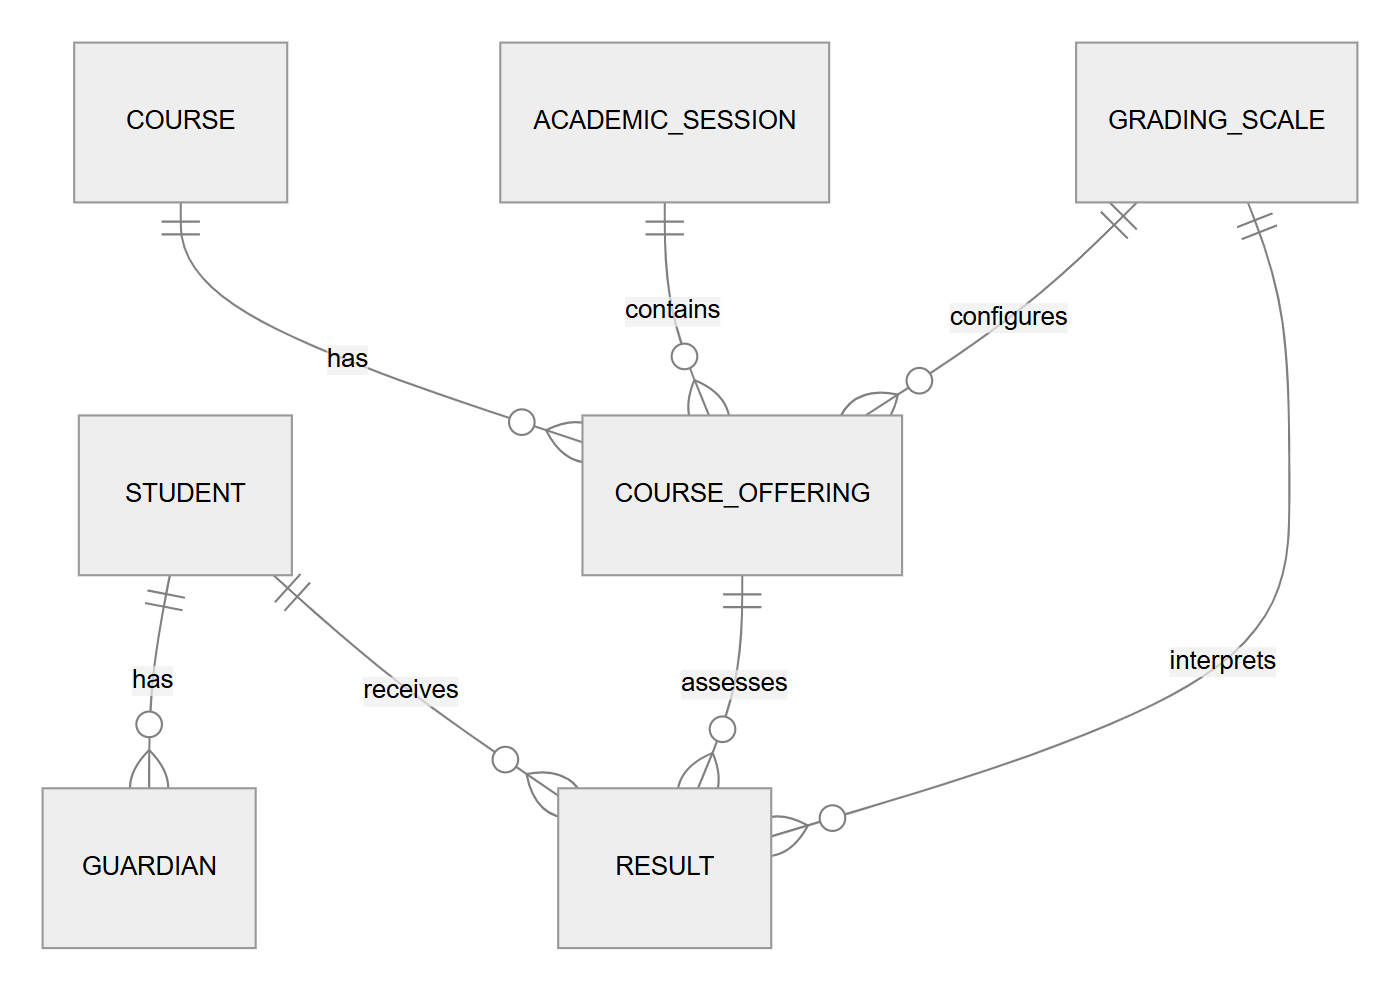
\includegraphics[width=\linewidth,height=0.78\textheight,keepaspectratio]{folder/figure-3_2-academic-records.png}
\caption{Selected student and academic record relationships}\label{fig:3-2}
\end{figure}
\clearpage

\subsection{Validation transactions and correction}\label{sec:3-4-2}

Validation is applied to the meaning and permitted range of inputs as well as their representation. Examples include valid academic periods, finite numerical scores, positive credit units and permitted changes to student information. Database constraints prevent specified duplicate identities, result attempts and attendance records. Application services add the permission and workflow checks required before a change is accepted.

Related updates use transactions where partial completion would create an inconsistent state. The current attendance and import services also use locks to coordinate competing operations. The purpose is to preserve a defined outcome when submissions, retries or permission changes occur concurrently. These mechanisms apply the constraint and transaction principles described by the PostgreSQL Global Development Group~\cite{pgconstraints,pgtransactions}; the specific workflow rules are properties of the project implementation.

A correction to structured information is distinguished from replacing a supporting document. Structured changes follow the relevant field and permission rules. A replacement document should retain a link to its preceding version and a reason for the change. Comprehensive audit recording and the proposed document-history mechanisms require further implementation; the presence of selected correction records does not establish an application-wide audit trail.

\subsection{Academic calculations}\label{sec:3-4-3}

The backend calculates grade-point averages from verified result records using saved credit units and the applicable published grading scale. The general expression is:

\begin{equation}
GPA=\frac{\sum_{i=1}^{n}u_i g_i}{\sum_{i=1}^{n}u_i},
\end{equation}

where \(u_i\) is the saved credit units and \(g_i\) is the grade point for result \(i\). Semester GPA uses the selected session and semester, while the implemented CGPA function uses the recorded cumulative attempts. Failed and repeated recorded attempts are included under the current project rule. This rule must be reconciled with authoritative departmental policy before being described as an official university calculation policy.


% !TeX root = ../main.tex
\begingroup
\singlespacing%
\setlength{\tabcolsep}{4pt}
\begin{longtable}{@{}>{\raggedright\arraybackslash}p{\dimexpr0.480\linewidth-2\tabcolsep\relax}>{\raggedleft\arraybackslash}p{\dimexpr0.520\linewidth-2\tabcolsep\relax}@{}}
\caption{Initial project grading configuration}\label{tab:3-3}\\
\toprule
\textbf{Score interval} & \textbf{Grade point} \\
\midrule
\endfirsthead%
\toprule
\textbf{Score interval} & \textbf{Grade point} \\
\midrule
\endhead%
\midrule
\multicolumn{2}{r}{Continued on next page}\\
\endfoot%
\bottomrule
\endlastfoot%
0 up to but excluding 40 & 0 \\ \addlinespace
40 up to but excluding 45 & 1 \\ \addlinespace
45 up to but excluding 50 & 2 \\ \addlinespace
50 up to but excluding 60 & 3 \\ \addlinespace
60 up to but excluding 70 & 4 \\ \addlinespace
70 through 100 inclusive & 5 \\ 
\end{longtable}
\endgroup


The implementation rejects invalid or missing scores in a supplied calculation set and requires verification of the supplied results. It returns no average where there are no results. A numerical CGPA is kept separate from academic completeness and graduation review. Independent worked examples, boundary values and incomplete-history cases form part of the evaluation procedure.

\section{Proposed Document Filing Subsystem}\label{sec:3-5}

\subsection{Metadata and revision design}\label{sec:3-5-1}

Uploaded documents are confirmed project scope, but their private storage and revision management are not yet established as implemented. The proposed design associates every document with the permanent student UUID and separates its descriptive metadata from the stored file. It also separates the continuing document identity from individual uploaded revisions.


% !TeX root = ../main.tex
\begingroup
\singlespacing%
\setlength{\tabcolsep}{4pt}
\begin{longtable}{@{}>{\RaggedRight\arraybackslash}p{\dimexpr0.220\linewidth-2\tabcolsep\relax}>{\RaggedRight\arraybackslash}p{\dimexpr0.390\linewidth-2\tabcolsep\relax}>{\RaggedRight\arraybackslash}p{\dimexpr0.390\linewidth-2\tabcolsep\relax}@{}}
\caption{Proposed document records}\label{tab:3-4}\\
\toprule
\textbf{Proposed record} & \textbf{Information to retain} & \textbf{Purpose} \\
\midrule
\endfirsthead%
\toprule
\textbf{Proposed record} & \textbf{Information to retain} & \textbf{Purpose} \\
\midrule
\endhead%
\midrule
\multicolumn{3}{r}{Continued on next page}\\
\endfoot%
\bottomrule
\endlastfoot%
Student\allowbreak~Document & Document UUID, student UUID, title, category, relevant academic period and current revision reference & Organises the continuing document within the student's file. \\ \addlinespace
Document\allowbreak~Revision & Revision UUID/sequence, document reference, original filename, internal storage key, detected file type, byte length and integrity digest & Identifies the particular uploaded content without using its public filename as an access mechanism. \\ \addlinespace
Revision provenance & Uploader, upload time, source description and replacement/correction reason & Explains how the document entered the system and why a later revision exists. \\ \addlinespace
Document state & Validation/review state and any approved archive or retention information & Prevents an incomplete or rejected upload being treated as an available record. \\ \addlinespace
\end{longtable}
\endgroup


The entity names in Table 3.4 are proposed design names, not existing Django models. Document categories, permitted formats, file-size limits, revision authority and retention periods remain configuration and policy decisions to finalise. Candidate categories can be derived from the actual departmental inventory rather than assumed to cover every type of university document.

\subsection{Upload and retrieval procedure}\label{sec:3-5-2}

The proposed upload workflow first authenticates the user and checks permission for the target student and document category. The uploaded file is staged while its size, detected type and content-validation requirements are checked. Descriptive metadata is validated, and an internal storage key associates the private file with the revision record. Only an accepted revision becomes available through authorised retrieval.

The design must coordinate storage and database failures. A database transaction cannot by itself make a separate filesystem write atomic. A staged upload therefore needs an explicit completion state and a cleanup or recovery procedure for interrupted publication. The evaluation will verify that an incomplete upload is not presented as a valid document and that failures do not produce a published record with missing content.

Retrieval begins with an authorised search of student and document metadata. Before download or display, the backend rechecks permission and resolves the internal storage key. Knowing a file path or document UUID should not bypass this check. A proposed replacement creates a new revision with a reason and actor; it does not silently overwrite the earlier revision or its provenance.

The first implementation can support metadata-based retrieval without claiming OCR or full-text search. If extraction of scanned document contents is later selected, it requires an additional recognition and validation procedure. The existing PDF results parser is a separate layout-specific tool and does not establish OCR capability for arbitrary scanned files.

\section{Access Control and Web Application Design}\label{sec:3-6}

The current application uses staff and student accounts with server-side action permissions and record scope. Ordinary adviser operations require the relevant permission and an active assignment for the current academic session and student level. Attendance operations additionally use explicit course assignments. A linked student account accesses the student's own permitted information. The active HOD account is represented through the application's privileged administration policy.


% !TeX root = ../main.tex
\begingroup
\singlespacing%
\setlength{\tabcolsep}{4pt}
\begin{longtable}{@{}>{\RaggedRight\arraybackslash}p{\dimexpr0.220\linewidth-2\tabcolsep\relax}>{\RaggedRight\arraybackslash}p{\dimexpr0.390\linewidth-2\tabcolsep\relax}>{\RaggedRight\arraybackslash}p{\dimexpr0.390\linewidth-2\tabcolsep\relax}@{}}
\caption{Selected access contexts}\label{tab:3-5}\\
\toprule
\textbf{User context} & \textbf{Records or activity context} & \textbf{Access condition} \\
\midrule
\endfirsthead%
\toprule
\textbf{User context} & \textbf{Records or activity context} & \textbf{Access condition} \\
\midrule
\endhead%
\midrule
\multicolumn{3}{r}{Continued on next page}\\
\endfoot%
\bottomrule
\endlastfoot%
HOD administration & Departmental configuration and permitted administrative operations & Active privileged staff identity and the relevant administrative workflow. \\ \addlinespace
Ordinary adviser & Student profiles and selected academic operations & Action permission plus active assignment in the current academic session and level. \\ \addlinespace
Assigned course staff & Attendance class, roster-related views and permitted recording/correction & Relevant attendance permission and active assignment to the course offering. \\ \addlinespace
Student account & Own profile and permitted verified results or attendance information & Active account linked to that student's profile; no general staff record access. \\ \addlinespace
Document user & A particular student's document/category & Proposed explicit document permission and scope; final category policy remains to be implemented. \\ \addlinespace
\end{longtable}
\endgroup


The implemented JSON API uses session authentication and CSRF controls for the relevant browser write requests. Input and permission checks occur in the backend even when the interface also provides validation. Browser screens require integration tests for authentication, loading, invalid input, denied access and successful record operations. Their final evaluation must use the connected application rather than screenshots or prototype state alone.

Supporting functions such as messaging, guardian information and selected result-sharing operations exist in the backend. Their inclusion in the final report should remain proportional to the filing and identification objectives and to the functions actually demonstrated. They do not substitute for testing the required records and document workflows.

\section{Hardware Configuration and Firmware Design}\label{sec:3-7}

\subsection{Tested components and interfaces}\label{sec:3-7-1}

The hardware records identify a regular ESP32-D0WD-V3 development board with 4 MB flash and an AS608-labelled fingerprint module whose internal firmware version is unknown. The scanner reports a reference capacity of 150 and was used at security level 3 with 57,600-baud UART communication. The PC serial recording interface uses 115,200 baud. Upload baud rate, scanner baud rate and console baud rate are separate settings.

The DS1307 clock was used for the recorded recognition pilot. The later deferred-capture firmware does not integrate its calendar-time path and deliberately retains null capture dates. Optional OLED, button and feedback configurations are described by the terminal design but should not all be presented as physically validated parts of the measured pilot.


% !TeX root = ../main.tex
\begingroup
\singlespacing%
\setlength{\tabcolsep}{4pt}
\begin{longtable}{@{}>{\RaggedRight\arraybackslash}p{\dimexpr0.220\linewidth-2\tabcolsep\relax}>{\RaggedRight\arraybackslash}p{\dimexpr0.390\linewidth-2\tabcolsep\relax}>{\RaggedRight\arraybackslash}p{\dimexpr0.390\linewidth-2\tabcolsep\relax}@{}}
\caption{Regular ESP32 interface configuration}\label{tab:3-6}\\
\toprule
\textbf{Interface or function} & \textbf{Configuration} & \textbf{Evidence status} \\
\midrule
\endfirsthead%
\toprule
\textbf{Interface or function} & \textbf{Configuration} & \textbf{Evidence status} \\
\midrule
\endhead%
\midrule
\multicolumn{3}{r}{Continued on next page}\\
\endfoot%
\bottomrule
\endlastfoot%
Scanner TX to ESP32 RX & GPIO16 & Working UART connection recorded in hardware tests. \\ \addlinespace
Scanner RX from ESP32 TX & GPIO17 & Working UART connection recorded in hardware tests. \\ \addlinespace
Scanner UART & 57,600 baud, 8N1 & Recorded scanner communication configuration. \\ \addlinespace
PC console/recorder & 115,200 baud & Firmware and recorder configuration. \\ \addlinespace
I2C SDA/SCL & GPIO21/GPIO22, 100 kHz & Configured bus used by the clock path; final assembly schematic must show actual connections. \\ \addlinespace
DS1307 address & 0\(\text{x}\)68 & Clock adapter configuration and pilot timekeeping. \\ \addlinespace
Optional SSD1306 display & \(128\times64\), configured address 0\(\text{x}\)3C & Optional adapter; inclusion in the final build needs its own evidence. \\ \addlinespace
Enrol/\allowbreak~delete/\allowbreak~menu buttons & GPIO25/\allowbreak~GPIO26/\allowbreak~GPIO27 & Regular-board UI configuration, separate from the accuracy and deferred-capture profiles. \\ \addlinespace
Green/red LED outputs & GPIO18/GPIO19 & Configured feedback outputs; actual parts and resistor values require final schematic evidence. \\ \addlinespace
Buzzer control & GPIO23 & Configured output; the proposed driver stage is not established as a measured assembled circuit. \\ \addlinespace
\end{longtable}
\endgroup


The regular ESP32's capabilities are documented by Espressif Systems~\cite{esp32}; ESP32-S3 specifications are not substituted for the tested board. The DS1307 datasheet specifies a 4.5--5.5 V device supply and standard-mode I2C operation~\cite{analogds1307}. The board-side bus must remain compatible with ESP32 logic levels; breakout pull-ups and any level translation belong in the final schematic. Actual supply rail and current measurements are still needed before a measured power budget or battery runtime can be reported.

For design analysis, an LED resistor can be selected from \(R=(V_{drive}-V_F)/I_F\) using the actual LED and drive limits. Average load power can be estimated from measured rail quantities as \(P_{avg}=\sum_k V_k I_{k,avg}\). Where a battery is implemented, an estimated runtime is \(t=E_{usable}\eta/P_{avg}\) when usable battery energy is defined before conversion. These expressions are design tools, not results from measurements already performed.

\subsection{Firmware separation and capture state}\label{sec:3-7-2}

The firmware uses C++ with the Arduino framework under PlatformIO\@. Separate build profiles support normal diagnostics, whole-gallery recognition evaluation, selected-slot evaluation and deferred unidentified capture. This separation preserves the experimental meaning of each mode. The accuracy builds do not create application attendance records, while the deferred profile disables the older local attendance UI\@.

The capture controller requires finger removal between presentations and records only a completed acquisition attempt according to its defined procedure. Communication commands use bounded waits and validated responses. Uncertain persistence is reported rather than automatically retried as a destructive change.

The general deferred-capture states are shown in Figure 3.3. Storage or recovery faults require attention; rebooted capture does not silently resume without explicit arming.

\begin{figure}[htbp]
\centering
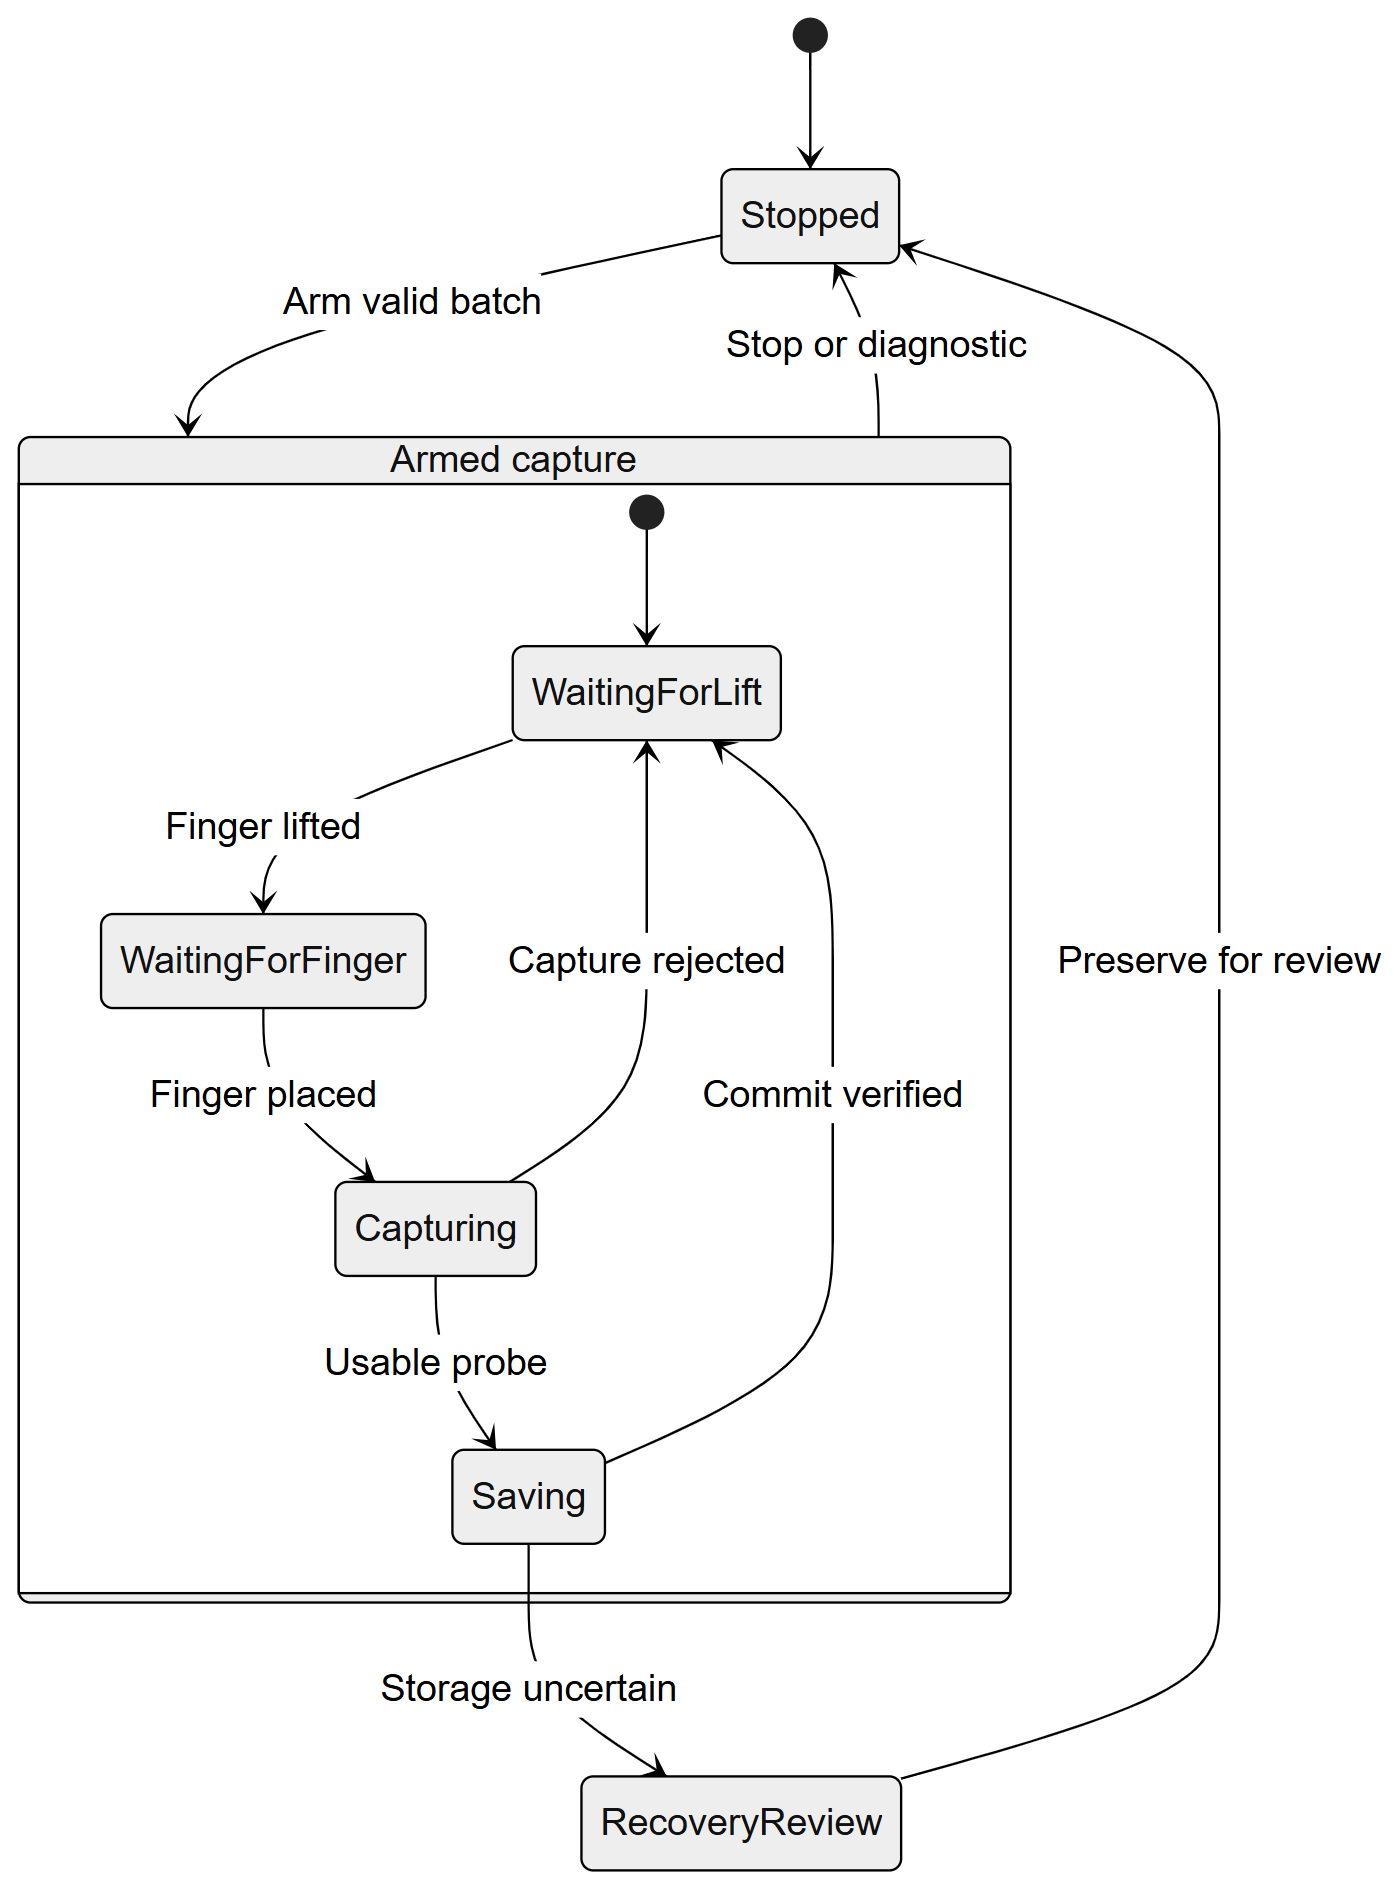
\includegraphics[width=\linewidth,height=0.78\textheight,keepaspectratio]{folder/figure-3_3-capture-states.png}
\caption{Simplified deferred-capture state model}\label{fig:3-3}
\end{figure}
\clearpage

The diagram is a behavioural summary. The implemented controller and recovery tests provide the detailed state transitions, timeouts and limits.

\section{Fingerprint References and Identity Integration}\label{sec:3-8}

\subsection{Enrolment and reference representation}\label{sec:3-8-1}

The diagnostic enrolment procedure acquires the presentations needed by the sensor to form a reference and stores it in a checked free slot. Normal diagnostic and accuracy-build enrolment use their documented procedure; the separate button UI contains an additional confirmation presentation and should not be described as the recognition pilot's enrolment protocol.

Reference transfer was implemented through the scanner's character-buffer and storage commands. The hardware log records a transferred opaque reference payload of 1,536 bytes, its saved integrity digest and readback checks. That observed length is not a universal specification for every scanner model, representation or UART packet. The project distinguishes the transferred payload from the transport packet size and from the number of occupied gallery slots.

The proposed enrolment registry associates a template/reference UUID with the student UUID, finger label, scanner/format compatibility information and gallery/slot binding. A local slot is a reference location that may change after restoration or library replacement. Exact-byte hashes detect content integrity; they are not used to recognise a person or to prove unique enrolment.

\subsection{Matching architecture and workflow decisions}\label{sec:3-8-2}

The saved recognition experiments perform comparison using the scanner. Later saved-probe feasibility work also used scanner-assisted direct comparison. A compatible software-only server matcher has not been established for the opaque representation. The integration design therefore leaves matching location and orchestration explicit: a backend can coordinate compatible comparison without implying that Django itself decodes the template or executes the sensor's proprietary algorithm.

For a resolved biometric outcome, the proposed workflow checks the active reference-to-student binding, the student's eligibility for the selected class and the authority of the operation. Unknown, conflicting, inactive or out-of-roster outcomes remain unresolved or are rejected for the specified reason. A successful scan is not automatically an attendance record.

The attendance foundation uses course offerings, HOD-confirmed rosters and per-class membership snapshots. The candidate list can suggest active students at the relevant level and students with a latest verified failed prior attempt; a failure is not treated as proof of current registration. Reviewed roster membership, rather than course credit units, establishes the class population used by the workflow.

\subsection{Selectable attendance configurations in one installed build}\label{sec:attendance-runtime-modes}

The regular ESP32 application provides two runtime attendance configurations in
one installed SH1106-capable firmware. Recompilation and reinstallation are not
required to change attendance type. The operator opens Attendance Mode, chooses
Immediate or Deferred, and confirms the choice. Start/Stop and Deferred Class
Batch are separate menu pages. Entering a menu stops deferred acquisition; the
operator must explicitly restart it. Both acquisition paths are mutually
exclusive clients of the scanner UART.\@

% !TeX root = ../main.tex
\begingroup
\singlespacing%
\setlength{\tabcolsep}{4pt}
\begin{longtable}{@{}>{\RaggedRight\arraybackslash}p{\dimexpr.19\linewidth-2\tabcolsep\relax}>{\RaggedRight\arraybackslash}p{\dimexpr.405\linewidth-2\tabcolsep\relax}>{\RaggedRight\arraybackslash}p{\dimexpr.405\linewidth-2\tabcolsep\relax}@{}}
\caption{Runtime attendance configurations in the unified terminal}\label{tab:attendance-runtime-modes}\\
\toprule
\textbf{Property} & \textbf{Immediate local matching} & \textbf{Deferred capture} \\
\midrule\endfirsthead%
\toprule
\textbf{Property} & \textbf{Immediate local matching} & \textbf{Deferred capture} \\
\midrule\endhead%
\midrule\multicolumn{3}{r}{Continued on next page}\\\endfoot%
\bottomrule\endlastfoot%
Identity decision & Scanner searches existing enrolled references during the presentation. & No identity decision at capture; compatible matching and review occur later. \\ \addlinespace
Stored output & Local timestamp, reference hash, slot, score and event identifiers in CSV. & Unidentified probe and batch/event/boot identifiers in verified ESP32 files. \\ \addlinespace
Required setup & Enrolled gallery, valid RTC and writable log storage. & Prepared class-session batch, compatible scanner and writable capture storage; no preloaded gallery required. \\ \addlinespace
Positive feedback & Attendance Saved after a verified local append; one short beep and green indication. & Capture Saved / Pending Match after commit; one short beep with both LEDs off. \\ \addlinespace
Duplicates & Current prototype: same template and local date. Final class-session binding remains outstanding. & Finger lift separates capture attempts; resolved student/class duplicates require later reconciliation. \\ \addlinespace
Runtime selection & Choose Immediate and confirm; Start/Stop controls acquisition. & Choose Deferred and confirm; select a prepared batch and explicitly start it. \\ \addlinespace
Persistence & Existing CSV history is retained across mode changes. & Committed files and selected batch are retained; reboot leaves acquisition stopped. \\ \addlinespace
Reference slots & Attendance uses volatile capture buffers and existing references; it creates no new enrolled slot. & Attendance uses volatile capture buffers and ESP32 files; it creates no enrolled slot. \\ \addlinespace
Website status & Local save is not a website attendance submission. & Import is pending evidence; it is not confirmation that a named student attended. \\
\end{longtable}
\endgroup


In immediate mode, a fresh presentation is compared against the scanner's
enrolled references. A valid DS1307 timestamp and a verified local append are
required before the terminal reports Attendance Saved. This checkpoint records
local check-ins and suppresses a repeated template on the same local date. It
does not yet implement the final student/class-session identity reconciliation;
the daily rule must not be described as a per-class attendance rule.

Deferred mode stores the unidentified feature probe on the ESP32 and reports
Capture Saved / Pending Match only after commit and readback checks. It does not
search or add a reference to scanner flash. A backend class-session batch is
prepared through the USB tool; the physical interface can select a prepared
batch and start or stop capture without reflashing or maintaining a laptop
connection during acquisition. The selected batch is retained across restart,
but capture is never automatically armed after a reboot. Calendar timing and
identity reconciliation retain the limitations described in Section~\ref{sec:3-9}.

Neither attendance configuration consumes a new permanent scanner reference
slot per presentation. Only enrolment or an explicit reference deployment writes
such slots. Starting or changing attendance mode does not erase reference
templates, old check-ins or pending probes. First-time student registration
remains a separate integration requirement: the enrolment template must pass
through the laptop bridge to an authorised backend student binding, with success
acknowledged only after the database commit. A sensor-only Enrolled message does
not establish that website registration has completed.

Feedback distinguishes verified local outcomes from pending evidence. Green is
reserved for confirmed sensor enrolment, a verified immediate check-in append,
or a verified deliberate fingerprint deletion. Startup, progress, mode selection,
clock configuration, export and deferred capture do not light green. In
particular, the rule concerns a verified operation, not whether enrolment has
occurred since the most recent boot: restored references can also produce valid
immediate matches. Appendix~\ref{app:design} specifies the event feedback,
confirmation behaviour and remaining integration states.

\section{Deferred Capture Transfer and Pending Ingestion}\label{sec:3-9}

The deferred design captures fingerprints without requiring a preloaded per-class reference gallery. The terminal stores each unidentified probe in a class-bound batch with stable device, batch, event and boot identifiers. Event timing is retained as boot-relative elapsed milliseconds. These values preserve sequence and timing evidence but are not converted into an invented calendar date.

The device uses LittleFS and staged writes. It writes pending content, closes and reads it back, commits it under a new filename and verifies the committed content before reporting a saved capture. CRC32 fields detect corruption in the binary records. An interrupted pending write blocks further capture until its condition is reviewed; valid committed data can be exported with a recovery flag.

USB export transfers a bounded stream to a PC, where the downloader checks count and integrity information and creates a JSONL interchange file. The device files are retained after download. Neither a successful download nor a backend receipt authorises deletion of the source captures.


% !TeX root = ../main.tex
\begingroup
\singlespacing%
\setlength{\tabcolsep}{4pt}
\begin{longtable}{@{}>{\RaggedRight\arraybackslash}p{\dimexpr0.280\linewidth-2\tabcolsep\relax}>{\RaggedRight\arraybackslash}p{\dimexpr0.720\linewidth-2\tabcolsep\relax}@{}}
\caption{Implemented interchange bounds and meanings}\label{tab:3-7}\\
\toprule
\textbf{Property} & \textbf{Implemented bound or rule} \\
\midrule
\endfirsthead%
\toprule
\textbf{Property} & \textbf{Implemented bound or rule} \\
\midrule
\endhead%
\midrule
\multicolumn{2}{r}{Continued on next page}\\
\endfoot%
\bottomrule
\endlastfoot%
Capture probe & Maximum 2,048 decoded bytes per event. \\ \addlinespace
Batch & Maximum 512 capture events. \\ \addlinespace
Backend import file & Maximum 2 MiB. \\ \addlinespace
JSONL line & Maximum 4,096 bytes. \\ \addlinespace
Append behaviour & New snapshots may append to the exact stored prefix; existing events retain content and order. \\ \addlinespace
Exact retry & Recovers the durable receipt for the accepted file snapshot. \\ \addlinespace
Conflict & Changed event content, reused event identity or inconsistent batch binding rejects the transaction. \\ \addlinespace
Capture calendar time & Null until trusted timing provision and review are implemented. \\ \addlinespace
Import effect & Pending evidence only; no automatic student identity, attendance, absence or warning. \\ \addlinespace
\end{longtable}
\endgroup


The backend provides authorised preview, import and metadata-listing operations. Preview checks the complete file without persisting it. Import revalidates permission, class binding, file digest, schema and conflicts before committing evidence and a durable receipt atomically. A preview digest binds the selected bytes; it does not replace authentication or prove the physical device's identity.

The proposed reconciliation stage follows ingestion. It requires a compatible identity-resolution procedure and explicit timing review before invoking an attendance operation. Until this stage is implemented, the captures remain pending. Device authentication, encrypted biometric storage and key management, retention rules and final operational hardening also remain unfinished.

\section{Software and Records Evaluation Procedure}\label{sec:3-10}

\subsection{Evaluation levels}\label{sec:3-10-1}

Evaluation is organised into record/service tests, database and HTTP integration tests, terminal experiments and complete user workflows. These levels address different questions. A unit or service test checks a defined operation and its resulting state. Database contention tests examine interactions between simultaneous operations. HTTP tests exercise authentication, request handling and response behaviour. Browser and physical integration tests establish behaviour beyond those isolated components.

The current evidence includes backend validation in isolated databases and separate hardware experiments. Document-management, connected browser tasks and complete biometric reconciliation require additional evaluation. The numerical outcomes of completed tests belong in Chapter Four; the procedures and scope are specified here.

\subsection{Implemented backend validation}\label{sec:3-10-2}

Backend tests use synthetic student and academic fixtures rather than live departmental records. The documented checks include record permissions, result calculations, validation, attendance services and pending capture ingestion. Database-specific checks were run against an isolated PostgreSQL 16.15 instance. This environment was separate from the shared departmental source database.

The pending-ingestion validation included competing transactions using independent connections. A coordinator checked that one transaction was genuinely waiting on a database lock before the competing operation proceeded. Cases covered identical imports, competing append/prefix snapshots, conflicting event reuse, permission revocation, session changes and rollback. This procedure tests defined consistency properties under bounded contention; it is not a sustained throughput benchmark.

The documented HTTP cases used actual login, CSRF, session cookies and the original JSONL request bytes. They included permitted ingestion, anonymous or invalid-CSRF requests, revoked access, interrupted uploads, retry after a discarded response, and a fresh application-process restart. These checks extend beyond forced-authentication service tests while remaining separate from browser interaction and field deployment.

\subsection{Proposed records and document task study}\label{sec:3-10-3}

The records-task evaluation will use a declared synthetic dataset containing distinct students, academic periods, valid and invalid result cases, and representative supporting documents. The dataset size and document categories must be recorded when the study is performed. Examples will include similar student names, missing information, duplicate identifiers and documents with replacement revisions so that success requires returning the correct information rather than merely any search result.

Each task will specify the requested information, expected student/document identity and permitted user context. A retrieval task ends when the correct required information is displayed or the correct document is opened. A correction task additionally checks the saved state and the retained history or verification requirements. Valid and invalid inputs will be evaluated separately.

Document tests will cover accepted and rejected files, metadata association, permitted download, denied direct access, revision replacement and interruption during upload publication. Tests of storage/database failure will verify that incomplete content is not exposed as a completed record. Archive and retention behaviour will be evaluated only after their policy and implementation have been established.

If a comparison with hard-copy filing is conducted, the manual and digital conditions will use equivalent record sets and lookup requests. The study will record operator preparation, starting conditions, completion rules and task order. Where the same operator performs both conditions, order and familiarity effects will be considered. Until this study is performed, no percentage retrieval improvement or measured workload reduction is claimed.

\section{Fingerprint Recognition Pilot Procedure}\label{sec:3-11}

\subsection{Participants references and experimental conditions}\label{sec:3-11-1}

A functional recognition pilot was conducted on 15 October 2026 using one participant, one enrolled finger and one designated un-enrolled finger. The scanner contained one freshly enrolled reference in slot 1. Both recognition modes used that same reference at security level 3 and the recorded scanner communication settings. Finger labels were supplied by the operator; they were not independently determined from the recorder output.

The pilot was designed to check operation under these conditions. It did not sample a departmental student population or establish identification among several enrolled identities. Repeated presentations of the same fingers are correlated observations and are reported as repeated attempts, not independent participants.


% !TeX root = ../main.tex
\begingroup
\singlespacing%
\setlength{\tabcolsep}{4pt}
\begin{longtable}{@{}>{\RaggedRight\arraybackslash}p{\dimexpr0.220\linewidth-2\tabcolsep\relax}>{\RaggedRight\arraybackslash}p{\dimexpr0.390\linewidth-2\tabcolsep\relax}>{\RaggedRight\arraybackslash}p{\dimexpr0.390\linewidth-2\tabcolsep\relax}@{}}
\caption{Recognition pilot design}\label{tab:3-8}\\
\toprule
\textbf{Property} & \textbf{Whole-gallery experiment} & \textbf{Selected-slot experiment} \\
\midrule
\endfirsthead%
\toprule
\textbf{Property} & \textbf{Whole-gallery experiment} & \textbf{Selected-slot experiment} \\
\midrule
\endhead%
\midrule
\multicolumn{3}{r}{Continued on next page}\\
\endfoot%
\bottomrule
\endlastfoot%
Firmware profile & esp32-accuracy-identify & esp32-accuracy-verify \\ \addlinespace
Scanner operation & Search over the reported reference range & Search restricted to the selected occupied slot \\ \addlinespace
Operating mode & 1:N identification & Claimed-reference 1:1 check using selected-slot Search \\ \addlinespace
Reference gallery & One enrolled template, slot 1 & Same enrolled template, slot 1 \\ \addlinespace
Genuine attempts & Ten new presentations of the enrolled finger & Ten new presentations of the enrolled finger \\ \addlinespace
Negative attempts & Ten presentations of the designated unenrolled finger & Ten presentations of the designated different finger \\ \addlinespace
Trial separation & Detected lift and minimum two-second cooldown & Detected lift and minimum two-second cooldown \\ \addlinespace
\end{longtable}
\endgroup


\subsection{Trial collection}\label{sec:3-11-2}

Before each run, the reference inventory and settings were checked and the intended genuine identity selected for the recorder. A genuine block and a negative block were then collected under the operator-declared ground truth. The gallery remained fixed during the run. The expected identity in the identification experiment labelled the correct result without limiting the gallery search.

Each automatic trial used a new presentation, one feature-generation operation and one Search transaction. A continuously held finger did not generate repeated presentation trials. The recorder captured trial identifiers, declared case, returned identity where available, decision, processing errors, raw accepted-match score and timing information. Invalid or unavailable score values were retained as unavailable rather than replaced with a fabricated zero.

The two firmware modes were run separately, and their observations were analysed with separate denominators. Earlier diagnostic captures and later saved-probe comparisons were not pooled into these runs. In particular, the selected-slot Search pilot was not relabelled as a statistical direct-Match experiment.

\subsection{Classification of outcomes}\label{sec:3-11-3}

For a genuine identification attempt, a returned identity matching the expected slot was classified as a correct acceptance. No match was a genuine failure, and an accepted wrong identity was also a genuine identification failure with an additional wrong-identity flag. A negative search returning an enrolled identity was a false positive. A completed negative search returning no match was a correct rejection.

In the selected-slot experiment, the selected reference defined the claimed identity. A contradictory identity outside that requested range was treated as a protocol error rather than a valid verification result. Acquisition, communication, sensor and unclassified errors were recorded separately from completed decisions.

The automatic recorder observes detected acquisition attempts. It does not independently prove how many physical placements were entirely undetected. Polling errors without an established presentation were retained separately, and the absence of a separate physical-placement ledger limits claims about total presentation coverage.

\subsection{Timing and calendar checks}\label{sec:3-11-4}

Two processing intervals were retained. The total processing interval began with the image-acquisition command and ended with the completed recognition result. Search time covered the Search transaction alone. Human waiting, the inter-trial cooldown and the subsequent RTC read were excluded from these processing intervals. These measurements therefore differ from a complete attendance transaction or an operator's record-retrieval task.

The DS1307 was synchronised from the PC separately for each run using Lagos local time, UTC+01:00. Trial-linked calendar readings and additional clock-status checks were recorded. Calendar sequence and differences from PC receipt time were inspected as functional checks. Serial and host delay, PC clock error and one-second calendar resolution prevent those differences from being treated as calibrated absolute clock accuracy or long-term drift.

\section{Reference Transfer and Deferred Capture Experiments}\label{sec:3-12}

\subsection{Reference transfer and restoration}\label{sec:3-12-1}

Reference portability was investigated separately from recognition accuracy. An enrolled reference was exported from the scanner, saved with its metadata and integrity digest, and restored through the supported buffer/storage commands. Readback was compared with the original bytes. The procedure distinguishes successful byte transfer from successful recognition and from compatibility with another physical scanner or software matcher.

The hardware record also documents an explicitly authorised erase/restore experiment after the occupied library and backup coverage had been checked. This historical procedure is reported as an experiment, not as a routine requirement for enrolment or evaluation. Scanner slots and gallery state were recorded so that a changed library could not be treated as the same experimental reference set without qualification.

\subsection{Saved-probe persistence and later comparison}\label{sec:3-12-2}

On 16 October 2026, the deferred firmware was used to acquire a live probe and preserve it in ESP32 storage under a synthetic class-session context. The batch was downloaded and validated, then downloaded again after an operator-reported USB power cycle. The saved outputs were compared for byte equality and integrity.

The saved probe was subsequently compared against the enrolled reference through scanner-assisted direct comparison. No new finger presentation was taken during that final comparison. This procedure evaluates preservation and subsequent usability of the saved representation. It is separate from the 15 October repeated-presentation study and is not a software-only server-matching experiment.

The physical check did not interrupt an unfinished flash write under a controlled brownout. Native storage and controller tests modelled interrupted-write and reboot states, but those tests are not described as measured electrical power-failure behaviour. The distinction is retained when discussing recovery results.

\section{Performance Measures and Analysis}\label{sec:3-13}

\subsection{Records and document measures}\label{sec:3-13-1}

For a defined set of assigned record tasks, task correctness is calculated as:

\begin{equation}
Task\ correctness=\frac{N_{correctly\ completed}}{N_{assigned}}\times100\%.
\end{equation}

A task is correctly completed only when the expected student information or document is returned and the required state is preserved. The test log records failures and denied operations separately so that a fast incorrect retrieval cannot count as successful performance.

For timing observations \(t_i\), the elapsed interval is \(t_i=t_{finish,i}-t_{start,i}\). User-task time, HTTP response time and database-operation time are labelled separately. Repeated task times will be summarised with the observation count, median and range or a suitable percentile. Document sizes and network conditions accompany upload/download measurements where they affect the interval.

If a comparable manual baseline is available, an indicative median time reduction can be expressed as:

\begin{equation}
Time\ reduction=\frac{\widetilde{t}_{manual}-\widetilde{t}_{digital}}
{\widetilde{t}_{manual}}\times100\%,
\end{equation}

provided the manual median is positive and the tasks and timing rules are comparable. This expression defines a planned analysis; no baseline value or improvement percentage has yet been supplied.

\subsection{Biometric decision measures}\label{sec:3-13-2}

The biometric analysis uses the trial definitions in Section 3.11 and the firmware's separate error counters. Let \(TP\), \(TN\), \(FP\) and \(FN\) denote completed decision outcomes. For genuine identification attempts, \(FN\) includes both no-match failures and wrong-identity decisions; the wrong-identity count is a subset and is not added a second time. Let \(N_{recorded}\) include all recorded attempts, including processing errors, and let:

\begin{equation}
N_{decision}=TP+TN+FP+FN.
\end{equation}

The following measures are then reported where their denominators are non-zero:

\begin{equation}
Decision\ accuracy=\frac{TP+TN}{N_{decision}}\times100\%,
\end{equation}

\begin{equation}
\begin{gathered}
Sensitivity\ or\ recall=\frac{TP}{TP+FN}\times100\%,
\\
Specificity=\frac{TN}{TN+FP}\times100\%,
\end{gathered}
\end{equation}

\begin{equation}
Decision\ coverage=\frac{N_{decision}}{N_{recorded}}\times100\%.
\end{equation}

Acquisition, communication, sensor and unclassified-error counts are also reported against the recorded-attempt denominator. They are not silently removed from the description of overall operation merely because completed-decision accuracy excludes them. A zero denominator produces an unavailable measure, not a zero error rate.

For the whole-gallery protocol, completed un-enrolled searches returning an enrolled identity define the false-positive identification rate:

\begin{equation}
FPIR=\frac{FP}{FP+TN}\times100\%.
\end{equation}

Completed genuine searches returning no match or the wrong identity define the stated top-one identification failure measure:

\begin{equation}
FNIR=\frac{FN}{TP+FN}\times100\%.
\end{equation}

These are protocol-defined identification rates, kept separate from the selected-slot decision rates. Verification/identification and threshold-dependent error terminology follow the distinction discussed by Fiumara~\cite{fiumara2022} and the biometric literature reviewed in Chapter Two.

The raw sensor matching score is retained only as supplementary comparison evidence. It is not converted into a probability, and accepted-only scores are not used to construct an unsupported equal-error rate or complete ROC/DET curve. Zero observed errors are reported as counts over the observed attempts rather than proof of a zero underlying error probability.

\subsection{Integration and reliability measures}\label{sec:3-13-3}

Integration evaluation checks whether each accepted operation creates the intended state and whether rejected or repeated inputs preserve it. Capture-import cases verify event counts, immutability, rollback and receipt identity. Once biometric reconciliation is implemented, each resolved event will be traced through identity binding, eligibility and timing checks to the final attendance operation.


% !TeX root = ../main.tex
\begingroup
\singlespacing%
\setlength{\tabcolsep}{4pt}
\begin{longtable}{@{}>{\RaggedRight\arraybackslash}p{\dimexpr0.220\linewidth-2\tabcolsep\relax}>{\RaggedRight\arraybackslash}p{\dimexpr0.390\linewidth-2\tabcolsep\relax}>{\RaggedRight\arraybackslash}p{\dimexpr0.390\linewidth-2\tabcolsep\relax}@{}}
\caption{Evaluation groups and required evidence}\label{tab:3-9}\\
\toprule
\textbf{Test group} & \textbf{Expected observation} & \textbf{Position in the present evidence} \\
\midrule
\endfirsthead%
\toprule
\textbf{Test group} & \textbf{Expected observation} & \textbf{Position in the present evidence} \\
\midrule
\endhead%
\midrule
\multicolumn{3}{r}{Continued on next page}\\
\endfoot%
\bottomrule
\endlastfoot%
Student identity and record integrity & Correct associations; prohibited duplicates and invalid references rejected & Existing backend tests; final evidence set to identify in Chapter Four. \\ \addlinespace
Academic calculations & Agreement with independent examples and correct handling of boundaries/missing data & Implemented calculation tests; institutional policy reconciliation remains separate. \\ \addlinespace
Access scope & Permitted requests succeed and prohibited requests disclose or change no protected information & Existing backend tests; browser interaction still requires evaluation. \\ \addlinespace
Document upload and publication & Valid content attached to the intended student; incomplete/invalid uploads not published & Proposed subsystem and tests. \\ \addlinespace
Document retrieval and revisions & Authorised retrieval, denied direct access and preserved replacement history & Proposed subsystem and tests. \\ \addlinespace
Recognition pilot & Per-trial correct/wrong identity, rejection, error and timing evidence & Recorded one-participant pilot with separate recognition modes. \\ \addlinespace
Reference/\allowbreak~probe preservation & Byte integrity across transfer, restoration or the stated restart procedure & Separate recorded hardware experiments. \\ \addlinespace
Pending ingestion and replay & Immutable evidence, atomic conflict rejection and durable retry receipts & Existing database and HTTP validation. \\ \addlinespace
Biometric-to-attendance reconciliation & Correct student/class association; no premature or duplicate attendance effect & Proposed remaining integration. \\ \addlinespace
Complete filing tasks and manual comparison & Correct user-task completion with consistently defined time & Planned; dataset and baseline need collection. \\ \addlinespace
\end{longtable}
\endgroup


Failure analysis records the initial condition, attempted operation, observed failure, resulting state and any subsequent correction. A passing synthetic regression, a physical terminal observation and a field result are distinct kinds of evidence. None is used as a substitute for an unperformed test at another level.

\section{Data Handling and Methodological Limits}\label{sec:3-14}

Initial software tests used synthetic fixtures. Biometric trial records and saved representations are retained in restricted local working storage and are not required in the public report. The report presents aggregate outcomes and non-sensitive metadata needed to understand the experiment. Document and biometric access, retention and eventual deletion require explicit policies as the system progresses towards operational use.

The present recognition study is limited by one participant, one enrolled reference and repeated presentations of two designated fingers. It does not test multiple-identity gallery selection or population error rates. Timing comparisons with other studies are also limited by different operation boundaries, scanners, datasets and retry procedures. The later saved-probe experiment establishes a different feasibility question and is discussed separately.

Additional volunteer studies will require a documented recruitment and consent procedure and the appropriate project approvals before data collection. Those procedures are not retroactively claimed for the current pilot. Live departmental source-data use and deployment are likewise separate from isolated synthetic validation.

The final power arrangement, physical enclosure fit, full document workflow, trusted timing for deferred captures, device authentication and complete biometric reconciliation remain development or evaluation work. These limits define the claims that can be made from the current prototype; they do not remove the corresponding requirements from the approved project scope.

\section{Traceability to the Project Objectives}\label{sec:3-15}


% !TeX root = ../main.tex
\begingroup
\singlespacing%
\setlength{\tabcolsep}{4pt}
\begin{longtable}{@{}>{\RaggedRight\arraybackslash}p{\dimexpr0.220\linewidth-2\tabcolsep\relax}>{\RaggedRight\arraybackslash}p{\dimexpr0.390\linewidth-2\tabcolsep\relax}>{\RaggedRight\arraybackslash}p{\dimexpr0.390\linewidth-2\tabcolsep\relax}@{}}
\caption{Relationship between objectives methods and report evidence}\label{tab:3-10}\\
\toprule
\textbf{Objective from Chapter One} & \textbf{Main methodology sections} & \textbf{Evidence for Chapter Four} \\
\midrule
\endfirsthead%
\toprule
\textbf{Objective from Chapter One} & \textbf{Main methodology sections} & \textbf{Evidence for Chapter Four} \\
\midrule
\endhead%
\midrule
\multicolumn{3}{r}{Continued on next page}\\
\endfoot%
\bottomrule
\endlastfoot%
Analyse the filing workflow and requirements & 3.2 and 3.3 & Dated local process evidence and requirements/access matrix. \\ \addlinespace
Design the records document and identity model & 3.4, 3.5 and 3.8 & ER/data dictionary, document design and tested integrity rules. \\ \addlinespace
Implement controlled web records and document functions & 3.4--3.6 and 3.10 & Connected operations, document cases, access results and filing-task observations. \\ \addlinespace
Implement the fingerprint terminal functions & 3.7, 3.8, 3.11 and 3.12 & Firmware/configuration, hardware evidence and defined recognition/preservation experiments. \\ \addlinespace
Integrate biometric identity with the selected workflow & 3.8, 3.9 and 3.13 & Identity binding, pending ingestion and final reconciliation cases, with unfinished links identified. \\ \addlinespace
Evaluate records biometrics and integration & 3.10--3.14 & Separate functional, timing, biometric and integration outcomes with limitations. \\ \addlinespace
\end{longtable}
\endgroup


\section{Chapter Summary}\label{sec:3-16}

The methodology translates the filing problem into structured records, supporting-document requirements, controlled web operations and a defined biometric integration path. It describes the implemented backend and terminal work, the recorded recognition and preservation procedures, and the proposed work needed for document management and complete identity reconciliation. The evaluation separates records correctness, biometric decisions and integration behaviour so that Chapter Four can report what each part demonstrates and where evidence remains incomplete.

